\documentclass[twoside]{article}
\usepackage{amsmath}
\usepackage{lipsum} % Package to generate dummy text throughout this template
\usepackage[english]{isodate}% http://ctan.org/pkg/isodate
\usepackage{pgfgantt}
\usepackage[show]{ed}
\setlength{\parindent}{0pt}
\usepackage[sc]{mathpazo} % Use the Palatino font
\usepackage[T1]{fontenc} % Use 8-bit encoding that has 256 glyphs
\linespread{1.5} % Line spacing - Palatino needs more space between lines
\usepackage{microtype} % Slightly tweak font spacing for aesthetics
\usepackage{minted}
\usemintedstyle{autumn}
\usepackage[hmarginratio=1:1,top=32mm,left=25mm,right=25mm,columnsep=18pt,bottom=27mm]{geometry} % Document margins
\usepackage{multicol} % Used for the two-column layout of the document
\usepackage[hang, small,labelfont=bf,up,textfont=it,up]{caption} % Custom captions under/above floats in tables or figures
\usepackage{booktabs} % Horizontal rules in tables
\usepackage{float} % Required for tables and figures in the multi-column environment - they need to be placed in specific locations with the [H] (e.g. \begin{table}[H])
\usepackage{hyperref} % For hyperlinks in the PDF
\usepackage{xspace}
\usepackage{lettrine} % The lettrine is the first enlarged letter at the beginning of the text
\usepackage{paralist} % Used for the compactitem environment which makes bullet points with less space between them
\usepackage{etoolbox}
\patchcmd{\thebibliography}{\section*{\refname}}{}{}{}
\usepackage{abstract} % Allows abstract customization
\renewcommand{\abstractnamefont}{\normalfont\bfseries} % Set the "Abstract" text to bold
\renewcommand{\abstracttextfont}{\normalfont\small\itshape} % Set the abstract itself to small italic text

\usepackage{titlesec} % Allows customization of titles
%\renewcommand\thesection{\Roman{section}} % Roman numerals for the sections
%\renewcommand\thesubsection{\Roman{subsection}} % Roman numerals for subsections
\titleformat{\section}[block]{\large\scshape\centering}{\thesection.}{1em}{} % Change the look of the section titles
\titleformat{\subsection}[block]{\large}{\thesubsection.}{1em}{} % Change the look of the section titles
\usepackage{cite}
\usepackage{fancyhdr} % Headers and footers
\pagestyle{fancy} % All pages have headers and footers
\fancyhead{} % Blank out the default header
\fancyfoot{} % Blank out the default footer
\fancyhead[C]{Naomi Pentrel $\bullet$ \href{mailto:n.pentrel@jacobs-university.de}{n.pentrel@jacobs-university.de} $\bullet$ \today} % Custom header text
\fancyfoot[RO,LE]{\thepage} % Custom footer text
\usepackage{graphicx}
\usepackage{wrapfig}

\usepackage{tocloft}

%\usepackage{csquotes}
%\MakeOuterQuote{"}

\hypersetup{
    bookmarks=true,
    unicode=false,
    pdftoolbar=true,
    pdfmenubar=true,
    pdffitwindow=false,
    pdfstartview={FitH},
    pdftitle={My title},
    pdfauthor={Author},
    pdfsubject={Subject},
    pdfcreator={Creator},
    pdfproducer={Producer},
    pdfkeywords={keyword1} {key2} {key3},
    pdfnewwindow=true,
    colorlinks=false,
    linkcolor=red,
    citecolor=green,
    filecolor=magenta,
    urlcolor=cyan
}

\usepackage{caption}
\usepackage{subcaption}
\usepackage[section]{placeins}
\usepackage{qtree}
\usepackage{gensymb}

\usepackage{setspace}

\usepackage{color}

%\doublespacing
% or:
%\onehalfspacing

%\renewcommand\cftchapafterpnum{\vskip10pt}
%\renewcommand\cftsecafterpnum{\vskip15pt}

%----------------------------------------------------------------------------------------
%	TITLE SECTION
%----------------------------------------------------------------------------------------

\title{\vspace{-15mm}\fontsize{24pt}{10pt}\selectfont\textbf{// All comments are NOT created equal}} % Article title


\newenvironment{myfont}{\fontfamily{\sfdefault}\selectfont}{\par}

%----------------------------------------------------------------------------------------
% Macros
%----------------------------------------------------------------------------------------
\newcommand{\sys}{\textsc{Knowtation}\xspace}

%----------------------------------------------------------------------------------------

\begin{document}
\thispagestyle{empty}
\pagenumbering{roman}
\begin{flushright}
    
\includegraphics[scale=1.0]{Logo}
  \end{flushright}
  \vspace{20mm}
  \begin{center}
    \huge
    \textbf{The Combination of Spatial Narrative and Semantic Closeness to derive Visualizations of Theory Graphs}
  \end{center}
  \vspace*{4mm}
  \begin{center}
   \Large by
  \end{center}
  \vspace*{4mm}
  \begin{center}
    \Large
    \textbf{Naomi Pentrel}
  \end{center}
  \vspace*{20mm}
  \begin{center}
    \large
    Bachelor Thesis Proposal in Computer Science
  \end{center}
  \vfill
  \begin{flushright}
    \large
    \begin{tabular}{l}
      
      \hline
      Prof. Dr. Michael Kohlhase \\
      \\
    \end{tabular}
  \end{flushright}
  \vspace*{8mm}
  \begin{flushleft}
    \large
    Date of Submission: \today \\
    \rule{\textwidth}{1pt}
  \end{flushleft}
  \begin{center}
    \Large Jacobs University Bremen - School of Engineering and Science
  \end{center}

\newpage
\noindent
  With my signature, I certify that this thesis has been written by me
  using only the indicates resources and materials. Where I have
  presented data and results, the data and results are complete,
  genuine, and have been obtained by me unless otherwise acknowledged;
  where my results derive from computer programs, these computer
  programs have been written by me unless otherwise acknowledged. I
  further confirm that this thesis has not been submitted, either in
  part or as a whole, for any other academic degree at this or another
  institution.

  \vspace{20mm}

    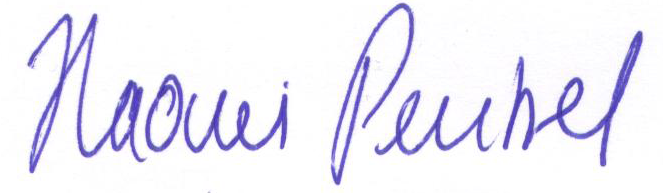
\includegraphics[scale=0.2]{Signature}
 \hfill Bremen, \today
  
\newpage

\thispagestyle{fancy} % All pages have headers and footers

%----------------------------------------------------------------------------------------
%	ARTICLE CONTENTS
%----------------------------------------------------------------------------------------

 \section*{Abstract}
Visualization of knowledge is important to foster learning. To optimize the visualization of information and its interdependencies, we will focus on identifying ways to present information without loosing context. The proposed research aims at taking an existing annotated corpus and presenting its contents in a way that allows the audience to see the dependencies of the covered topics. This form of presenting knowledge should enable users to examine materials they may have forgotten which form the basis for the understanding of the topics the audience is interested in.\\

Consider the typical lecture one attends as a student. Towards the end of the lecture students might have difficulties remembering earlier topics. When a new topic is introduced it would be ideal to have a simple way to find the dependencies and present students with a simple way to catch up.\\

The OMDoc (Open Mathematical Documents) format \cite{Kohlhase:OMDoc1.2} is a content markup scheme for mathematical documents. Using OMDoc, this research aims to visualize the connections of Mathematical knowledge in a way that allows students to learn the concepts the current topic depends on should they need to refresh their memories. As such it will foster learning and could transform how we interact with course material as a whole. This research has many other real world applications, namely, anywhere where knowledge is supposed to be transferred.\\ 

  \newpage
  \tableofcontents

  \clearpage
  \pagenumbering{arabic}

  \section{Introduction}

The intention behind the Semantic Web \cite{BernersLee:tsw98} is to transform the World Wide Web (WWW) from a web of mere human readable information to an information web with relations between different resources. There are an interesting similar developments in other fields such as that of new presentation tools. These aim to enable the presentation of information in a more interconnected way that provides context. Both developments strive to connect pieces of information and through providing context to elevate pure information to knowledge.\\

The concept behind these two developments is quite similar. Looking at the history of the WWW, specifically at the era of Web 2.0 \cite{Weller:npentrel14}, we notice that the web changed from an entity that only few people could add information to, to an entity that enables everyone to generate content. Whereas this lead to a lot of information on the web, it provided comparatively little knowledge. Here the processing of information to provide knowledge is lacking. Similarly the existence of tools like Powerpoint have lead to virtually everyone doing presentations in this format. As everyone who has witnessed many of these presentations knows, these are often easily compared to blogs: they contain some pieces of information but are often badly delivered and lack structure and context. \\

In essence, both issues stem from information being generated without enough context or structure. This makes the information hard to process by humans and/or machines. The Semantic Web hopes to change the former, whereas new, more visual presentation tools using spatial narrative, provide a framework for the creation of presentations that are easier to process for humans and thus facilitate knowledge transfer. The work proposed here intends to provide a tool for automatic contextual visualization of information through the usage of spatial narrative and semantic closeness of information. It adapts some of the concepts of the semantic web on a smaller scale.\\

\begin{center}
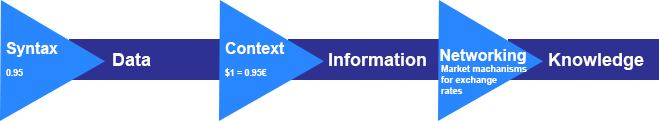
\includegraphics[scale=0.5]{model}
\end{center}

"Knowledge is the information necessary to support intelligent reasoning." \cite{Kohlhase:Complog:base} That said, it is imperative to facilitate knowledge transfer. The above graph is based on \cite{ProbstRaubRomhardt} and \cite{Kohlhase:Complog:base}. It shows the path from mere data to knowledge through adding context such that we gain information and then through adding networking to get knowledge.\\
\newpage
We want to go from merely displaying information to visualizing information by displaying the network/context a piece of information is in. In this we will not try to semantically represent the meaning of the information that is shown but rather on showing the network, i.e. the context the information is in. Specifically we want to examine whether spatial narrative can be combined with inherent semantic closeness of different pieces of information to facilitate knowledge transfer.\\

To achieve this goal, we intend to create a knowledge presentation system \sys to visually present information and its context (and networks). For this we will be using the OMDoc (Open Mathematical Documents) format which will provide us with an annotated set of documents. This will give us information about the semantic closeness of different pieces of information. From there on we will visualize the dependencies of the information contained in these documents. Of course we will not visualize the dependencies as a simple graph but use the approach of spatial narrative in the form of an API such as Impress.js to allow for us to show the current piece of information of interest within the network of dependent information.\\

To exemplify this: Annie, a young student learning Math, is watching her teacher give a presentation on how to use the Pythagorean theorem. She is given a triangle with sides a = 3 cm and b = 4 cm. Now she wants to use the theorem to calculate the length of side c. Annie already knows how to calculate the square of a number and thus calculates that $c^2 = 25 \implies c = 5$. However Annie made a mistake and did not know what a right triangle is. Her teacher tells her that the question was a trick question and that the answer is wrong because the triangle she calculated this for is not a right triangle. Now Annie has to try to find out what a right triangle is. This shows the dependencies of different pieces of information, i.e. the Pythagorean theorem depends on knowledge of squares, lengths, area calculation, angles, and right angles. In an ideal presentation this information should have been linked to the current piece of information so that Annie could have directly looked it up instead of having to search for it.\\

After reading this contrived story, I leave the reader to think about examples in his or her own life where he or she would have appreciated having the context of the information he or she was learning at the time. Many of these stories exist in real life and it is therefore important to provide this context to facilitate learning and knowledge transfer as a whole. \\

\section{Preliminaries}
To understand the problem of information that lacks context, this part will provide the necessary background information to allow us to derive a possible solution. While doing so it will demonstrate why this research is important and how it will improve the transfer of knowledge.\\

\ednote{This part should make clear which question, exactly, you are pursuing, and why your project is relevant/interesting. This is the place to cite relevant literature. Where does your project extend the state of the art? what weaknesses in known approaches to you hope to overcome? If you have carried out preliminary experiments, describe them here.}

\ednote{(target size: 3-4 pages)}
\ednote {explain primitives and apply to prezi.}

\subsection{Terminology}
Information 
Knowledge
Context.

\subsection{OMDoc}
OMDoc (\textbf{O}pen \textbf{M}athematical \textbf{Doc}uments) \cite{Kohlhase:OMDoc1.2} is an XML-based system that provides a data model and a format for content markup for mathematical documents. As such it is a semi-formal domain ontology. An ontology provides the framework for creating a semantic structure. It formally describes concepts within a specified area. A semi-formal ontology \cite{Sheth:npentrel14} is an ontology where formality of semantics is not a given. The semi-formal ontology can consist of partial or incomplete knowledge. \\

If OMDoc was used in every part of mathematics (and related fields), we would have a repository of mathematical knowledge that could be processed in different ways. This is possible because OMDoc provides the framework to create and store mathematical objects such as definitions and concepts. The relations between different mathematical objects and the attributes of mathematical objects can be added through annotations. This elevates the net of separate pieces of information that are stored individually to a semantic representation and one step further to knowledge.\\

In \cite{LK:MathOntoAuthDoc09} it is stated that "documents consist of narrative and content layers". The content layers are the mathematical objects, i.e. the statements or theories. Narrative layers refer to the order the mathematical objects from content layers are presented. In the proposed research the mathematical knowledge will be processed and visualized in a way that enables students to learn more efficiently. Thus it will not only provide the information or provide a narrative but it will provide a more interactive approach to presentations and learning.\\

\subsection{Status of Information within Discourse}
\ednote{intersection of knowledge of student and teacher aka shared knowledge base (also called “content commons”)}
In linguistics the concept of information packaging \cite{CambridgeGrammar:npentrel14} is known. Within this, one discriminates between \textit{familiar} and \textit{old} information. \textit{Familiar} information is shared by speaker and addressee, ie. common ground, whereas new information not. In addition one distinguishes information that is old or new with respect to the discourse or with respect to the addressee.\\

[1] \textit{"My sister went to the circus the other day; \underline{she} said \underline{it} was brilliant."}\\

In this example in the first part of the sentence information pertaining to my sister and to a circus are introduced, i.e. \textit{discourse-new}. In the second part the underlined parts are considered \textit{discourse-old} since they have already been introduced.\\

These concepts can be adapted to the situation of teaching Mathematics or Computer Science to students in a class. In general the information that the speaker is sharing with the addressees/students is \textit{discourse-new}\ednote{call course-new?} and depend on  information that is \textit{discourse-old}. I would like to introduce the term \textit{discourse-ancient} which covers the situation where the addressee has difficulties following the speaker since the \textit{discourse-new} information depends on \textit{discourse-old} information that might be 'too old', i.e. ancient, to be easily remembered.\\
\ednote {- reference old example from introduction -> and add onto it showing discourse-ancient.}

\subsection{Primitives}

Within knowledge representation, five evaluation criteria for knowledge representation are known \cite{Kohlhase:Complog:base}: Expressive Adequacy, Reasoning Efficiency, Primitives, Meta-representation, and Incompleteness. Primitives are the different elements of representation. In terms of evaluation it is important to have intuitive primitive elements. \\

For Impress.js, the primitive elements are text, images, frame-like structures, and the visual relation between the different frame-like structures. \ednote {not sure whether I understand this correctly}


\subsection{Context}

Context can be easily explained with the example of Annie learning the Pythagorean theorem. The information about the calculation of the length of the third side of the triangle is only helpful for Annie within the context of the pieces of information this depends on, i.e. calculating squares, lengths, area calculation, angles, and right angles. This is the context that the Pythagorean theorem needs.\\

Within this regard one should also consider context-sensitive and context-opaque\ednote{cite} information.  

\subsection{Spatial Narrative}
The development of of presentation tools like Impress.js and Prezi, "a virtual whiteboard that transforms presentations from monologues into conversations: enabling people to see, understand, and remember ideas" \cite{Prezi:npentrel14}, has  changed how people think about presentations. When doing a good prezi presentation one has to understand the topic one is presenting and think about how one can portray connections between content visually.\\

The concept of Spatial Narrative \cite{SpatialNarratives:npentrel14} stems from the establishment of frameworks for "the creation of computer-assisted flexibile 'guided tours' based on the thematically and narrative linking of a set of locations within an area into a 'spatial narrative'". An example for this is the experience of a tour guide for a certain topic.\\

The benefits of spatial narrative is that the audience gains a more thorough understanding of the subject and has a better understanding of the interconnections between different pieces of information. By providing the audience with a story as a narrative one also makes use of the concept of Storytelling which is largely accredited with the benefit that the audience will have an easier time following the presenter. That is because our brains are not made to memorize a lot of unconnected pieces of information; it is far easier for us to remember information if it comes in story form. \ednote{find source}\\

In this research we will use this knowledge to form an interconnected web of information that tells a visual story to facilitate the transfer of knowledge.

\subsection{Different Representations of Data}
What's the best representation one could do?
(1 page)
Forming Visualizations out of Knowledge Graphs which Convey Meaning
Meaningful Representation of Knowledge Graphs

\ednote{evaluation criteria from lecture slides}
\ednote{add how to work packages. -> my first approach will be...}
\newpage

\section{Work Plan}
\ednote {Add some speculation HOW}
\subsection{WP1: Understand API of Impress.js}
\ednote {should Impress.js go into the introduction/preliminaries? - I decided against this as I haven't examined Impress.js enough yet.}
The first step to implementing a \sys \ednote{Is the font format ok?} is to understand the tool we want to represent the knowledge in later. Since Prezi at the current time does not have an API that would allow for the generation of a whole presentation without the editor, this research will employ another tool that is inspired by the idea behind Prezi. Bartek Szopka's \textbf{Impress.js} \cite{JSImpress:npentrel14} is an open-source presentation framework which is based on CSS3 transforms and transitions. \ednote{Impressionist and jimpress}\\

\subsection{WP2: Using OMDoc to create ordered information graphs}
The idea is to use the General Computer Science Lecture notes \cite{Kohlhase:GenCSI:base} as an experiment. The General Computer Science Lecture notes are an annotated set of documents. Using OMDoc, we will create an information graph out of the annotated set of documents. This information graph should be ordered based on dependencies of knowledge.\\



\subsection{WP3: Combining OMDoc and Spatial Narration}
Once we have an ordered information graph we will visualize the information in different ways and analyze each way. The outcome of the analysis should be a model which we will then use to visualize the information in WP4.\\

\subsection{WP4: Implement OMDoc examples in Impress.js}
After the best model for spatial narration is found, we will implement a system that will take the ordered information graph and transform it into a spatial presentation using Impress.js.

\subsection{WP5: Evaluation}
Once we have examples, we will undertake a qualitative analysis of the visualization produced by the implemented \sys . In addition we will determine whether the implemented \sys meets the goals outlined in the Evaluation Criteria. Lastly we will measure the speed of the system.

\section{Evaluation Criteria}
\ednote {KEEP - real question: does spatial narrative work together with inherent semantic closeness -cogn. question: how does the spatial narrative work - should we use the inherent semantic closeness
}
\ednote {- work out concepts not a binding contract.}
\ednote{ 1. - 2. system goals -> kinda measurable}
\ednote{ 3.-5. cognitive goals -> exploring space of information systems}

\ednote{ make 2nd eval criteria last}

The evaluation criteria for the research at hand are on the one hand systematic and on the otherhand cognitive. Systematically we will be evaluating two main challenges: First we will evaluate whether the \sys that was developed allows for the creation of a full presentation from a given annotated document. Then we will evaluate the speed of the \sys . Special attention will be given to the question whether this could be used in real time such that a student could request a presentation on a certain topic and could this be generated on the fly within seconds.\\

Cognitively we will be examining whether the developed system provides a better system for knowledge transfer. For this a qualitative analysis will be conducted. Based on that we will be able to understand the positive and possibly negative effects of the combination of Spatial Narrative and OMDoc. 

\ednote{I am missing SMART goals... Can I use a scale from 0 - 10 for each point?}

If the implemented \sys can create a clearly structured presentation from a given annotated document that provides a better knowledge transfer experience, this research will be a full success. If this should fail and we know why it did not or cannot work the research will have succeeded in exploring an interesting way of trying to improve knowledge transfer and will serve to show future researchers what is impossible. \\

A stretch goal of this project is to have this research accessible for common users that could use it to create their own presentations. It is not the goal of this research that users should be able to reconstruct the original graph from the presentation.

\ednote{(target size: 1-2 page)}
\newpage
  \section{Timeline}

\textbf{Milestones}
\begin{itemize}
\item \textbf{Until February 1st}: Understanding the API of Impress.js
\item \textbf{Until March 1st}: Complete the creation of ordered information graphs using OMDoc
\item \textbf{Until March 15th}: Find an ideal model for the visualization of the information graph
\item \textbf{Until April 15th}: Implement/Automate the visualization of the information graph
\item \textbf{Until May 10th}: Qualitative Analysis and evaluation of findings 
\end{itemize}

\ednote {wp 4 - thesis writing}

\begin{figure}[h]
\begin{center}
\begin{ganttchart}[y unit title=0.4cm,
y unit chart=0.5cm,
vgrid,hgrid, 
title label anchor/.style={below=-1.6ex},
title left shift=.05,
title right shift=-.05,
title height=1,
bar/.style={fill=gray!50},
incomplete/.style={fill=white},
progress label text={},
bar height=0.7,
group right shift=0,
group top shift=.6,
group height=.3,
group peaks={}{}{.2}]{24}
%labels
\gantttitle{Proposed Timeline}{24} \\
\gantttitle{December}{4} 
\gantttitle{January}{4} 
\gantttitle{February}{4} 
\gantttitle{March}{4} 
\gantttitle{April}{4} 
\gantttitle{May}{4} \\
%tasks
\ganttbar{WP 1}{2}{8} \\
\ganttbar{WP 2}{9}{12} \\
\ganttbar{WP 3}{11}{14} \\
\ganttbar{WP 4}{15}{18}\\
\ganttbar{WP 5}{19}{21.5}
%relations 
\ganttlink{elem0}{elem1} 
\ganttlink{elem1}{elem2} 
\ganttlink{elem2}{elem3} 
\ganttlink{elem3}{elem4} 
\end{ganttchart}
\end{center}
\caption{Gantt Chart}
\end{figure}

  \section{Conclusions}

  Summarize the main aspects of the proposal.

  (target size: 1/2 page)

\newpage
\section{References}

\ednote{Research field: information systems}

\bibliography{kwarc}{}
\bibliographystyle{alpha}
\end{document}